\documentclass{article}

\usepackage[margin=1in]{geometry}
\usepackage{comment}
\usepackage{graphicx}
\usepackage{enumitem}
\usepackage[skip=7pt, indent=0]{parskip}
\usepackage{biblatex}
\addbibresource{isye_refs.bib}
\usepackage{hyperref}
\hypersetup{
colorlinks=true,
linkcolor=blue
}

\begin{document}
\clearpage\thispagestyle{empty}
\centering
\vspace{1cm}
    
\rule{\linewidth}{1mm} \\[0.5cm]
{ \Large \bfseries ISyE 6740 - Fall 2024\\[0.2cm]
    Final Report - Group 232}\\[0.5cm]
\rule{\linewidth}{1mm} \\[1cm]

\begin{tabular}{l p{5cm}}
\textbf{Team Member Names:} Michael Southard and Mustafa Alsaeedi &   \\[10pt]
\textbf{Project Title:} Where do healthy people live in the US? &  \\[10pt]
\end{tabular} 

\begin{itemize}[leftmargin=0pt]
\item[] \textbf{Problem Statement}
\begin{itemize}
    \item[] Understanding key factors correlating with positive health outcomes is important for driving public health policy. Here, we examine factors such as income, access to food (both "healthy" and "unhealthy" options), and access to recreational space and their relationship with health indicators such as diabetes rate, heart disease mortality, and life expectancy on the county level. We will also look for signs of racial/ethnic bias in access to health while controlling for potential differences in income. Our findings could function as an initial step towards government funding for public recreational areas, local farmers and markets, and/or grocery stores in counties lacking access.
\end{itemize}

\item[] \textbf{Background} 
\begin{itemize}
    \item[] In a 2010 editorial titled “How Healthy is Your County?”\cite{nash2010how}, David Nash provides an overview of a set of public health reports called “County Health Rankings”\cite{rwjf2010how} published by the Robert Wood Johnson Foundation, aimed to “aid public health and community leaders, policymakers, consumers, and others to see how healthy their county is, to compare it with others within their state, and to find ways to improve the health of their community.” 

    Amongst many other relationships, these reports found that 80\% of the least healthy counties were rural\cite{trapp2010health}, and healthier counties tended to be better educated and have greater access to healthful foods and recreational areas. David Nash also noted that there are many complex social and cultural factors that must be understood and addressed “to truly improve the health of our counties.”\cite{nash2010how}  

    Our goals for this project were to further substantiate the above findings through statistical modeling, gain insight into the complex social and cultural aspects of health (particularly racial/ethnic bias), and possibly uncover other relationships not mentioned in the above reports.  

    Disclaimer: We acknowledge that we are not experts in public health and it is very likely that new studies have emerged since 2010 that discuss/expand upon the relationships we will examine in this project.
\end{itemize}

\item[] \textbf{Data Sources}
\begin{itemize}
    \item \textit{See \hyperref[ref:bib]{References} and \hyperref[ref:fea]{Appendix} for additional information.}

    Our primary dataset comes from the USDA "Food Environment Atlas" (FEA)\cite{usda_food_environment_atlas}. This dataset contains many useful variables at the county level, including socioeconomic factors, health factors, store access, restaurant availability, farms and markets, and recreational facilities.

    We also used the following dataset for supplementary information:
    \begin{itemize}
        \item[] "Heart Disease Mortality Data Among US Adults (35+) by State/Territory and County": contains heart disease mortality rates by county, gender, and racial/ethnic group (2013-2015, 3-year average)\cite{heart_disease_mortality_data}
    \end{itemize}
\end{itemize}



\item[] \textbf{Methodology}
\begin{itemize}
\item[] \textbf{\textit{Data Preparation}} 

\item[] \textit{Data Aggregation}
\begin{itemize}
\item[] To initiate our dataset, we selected 43 features from the FEA “StateAndCountyData” csv file and aggregated them by county. We then merged this dataset with the 2010 Census Population variable in “SupplementalDataCounty.csv” and the Data\_Value variable from \\“Heart\_Disease\_Mortality\_Data\_Among\_US\_Adults\_\_35\_\_\_by\_State\_Territory\_and\_County.csv”, incorporating only the overall heart disease mortality data. Future analysis could further examine heart disease mortality by gender and racial/ethnic group, which is also provided in this file. 
\end{itemize}

\item[] \textit{Response Variable Selection}
\begin{itemize}
    \item[] We used principal component analysis (sklearn PCA) to perform dimensionality reduction on adult diabetes rate and heart disease mortality, resulting in a response variable that had a correlation coefficient of 0.89 with both diabetes rate and heart disease mortality, and explained 79.9\% of the variance in these features. We then scaled this response variable by –1 so positive values would indicate better health (lower diabetes rates and heart disease mortality), whereas negative values correspond to worse health outcomes at the county level. This variable will be referred to as “Health Score” throughout this paper. 
\end{itemize}

\item[] \textit{Collinearity}
\begin{itemize}
    \item[] Redundant collinear variables with correlation coefficients $>$0.8 were dropped from statistical modeling analysis or were combined with other variables to form the following ratios: 

    \begin{enumerate}
        \item "healthy\_store\_ratio" = ratio between stores with "healthy" options (grocery + specialty + supercenters) : stores without healthy options (convenience).
        \item "healthy\_restaurant\_ratio" = ratio between full service : fast food restaurants. 
        \item "recfac\_pc" = recreational facilities per capita (RECFAC11 / 2010\_Census\_Population) 
        \item "fmrkt\_pc" = farmers markets per capita (FMRKT13 / 2010\_Census\_Population)
        \item "sum\_farms" = sum(ORCHARD\_FARMS12, BERRY\_FARMS12, GHVEG\_FARMS12,\\ VEG\_FARMS12, CSA12, AGRITRSM\_OPS12) 
    \end{enumerate}
\end{itemize}

\item[] \textit{Nan Analysis}
\begin{itemize}
    \item[] We removed all variables that consisted of $>$5\% nans besides features that related to 2010 Census Population. Then, we removed all counties with remaining nans, resulting in a dataset consisting of 2920 counties, 93.11\% of the total number before nan removal. 
    \item[] We then compared the counties that were removed versus those retained and found a statistically significant difference in diabetes rates between the groups (t-test, p-value $<$ 0.001), where counties with incomplete data had diabetes rates between 0.96-1.64 percentage points higher than counties with complete data (\hyperref[fig:nan_bias]{see Appendix}). This bias warrants further examination, as it may indicate that less healthy counties may not have equal access to government and academic resources and attention.
\end{itemize}

\item[] \textit{Normality}
\begin{itemize}
    \item[] Many of the variables in this dataset appeared to be exponentially or Poisson distributed, and others had bimodal distributions or lacked a clear pattern. To make this data suitable for linear regression, we converted bimodal features into dummy variables and used quantile transformations (sklearn QuantileTransformer) to coerce the remaining features into (approximately) normal distributions. Some applications in this project use the transformed dataset and others use the raw data, depending on the model assumptions and application purpose. 
\end{itemize}

\item[] \textbf{\textit{EDA}}

Our exploratory data analysis consisted mainly of visualizing linear trends for numerical variables (Seaborn regplot) and distribution differences for categorical variables (Seaborn boxplot). 

\item[] \textbf{\textit{Detrending}}

Based on our EDA, we found strong relationships between health and income/age structure at the county level. These relationships were expected, and our goal was to look for more complex interactions that could help inform beneficial policy or behavioral changes. To help uncover any such relationships, we detrended our response variable (Health Score) by subtracting the predictions from a linear model (sklearn LinearRegression) fit using the following income- and age-related variables: median household income, poverty rate, \% households with low access to stores and have no vehicle, SNAP participants per 1000, \% 65 and older, and \% 18 and younger. This model had an R2 of 0.483 (\hyperref[fig:detrend]{see Appendix}). 

\item[] \textbf{\textit{Data Partitioning}}

We standardized and partitioned the data with a 70-30 train-test split (sklearn StandardScaler and train\_test\_split) before fitting the following LassoCV, OLS, and RandomForestRegressor models. The training sets were used for alpha selection and all model fitting, and the OLS and RandomForestRegressor test R2 scores were calculated on the test set.

\item[] \textbf{\textit{Feature Selection}}

After removing the income and age structure features, we had 16 features remaining for further exploration (\hyperref[fig:lassocv]{see Appendix}). Using the normalized data, we performed feature selection with LASSO regression, using 10-fold cross validation to select an appropriate alpha parameter (sklearn LassoCV, see appendix). LASSO regression did not remove any features from the model. 

\item[] \textbf{\textit{Health Models}}

We used linear regression (statsmodels OLS) and random forest (sklearn RandomForestRegressor) models to examine the relationship between detrended health score and race/ethnicity, access to healthy foods, food taxes, and a few other variables. Default parameters were used for both models, as increasing n\_estimators did not appear to improve random forest OOB score. The model results, including training and testing R2, coefficients, and Gini importance can be found in \hyperref[fig:statsmodelsOLS]{Appendix}. We also checked that the linear regression residuals were approximately normal and did not display heteroskedasticity.

For context, we also fit a random forest model using raw data (before nan removal, normalization, and detrending) to gauge the maximum proportion of variance in Health Score that could be explained by our dataset. This model used 150 estimators and had a test R2 of 0.737. Median household income was by far the most influential feature by Gini importance.

\item[] \textbf{\textit{Race/ethnicity Clustering}}

To further explore the relationship between health and race/ethnicity, we used k-means clustering (sklearn KMeans) to group similar counties in terms of \% white, \% black, and \% Hispanic populations. The highest silhouette score occurred with 3 clusters (\hyperref[fig:kmeans_scores]{see Appendix}); and upon visual inspection, 3 clusters seemed to partition the data well (\hyperref[fig:kmeans_pairplot]{see Appendix}). K-means clustering effectively separated the counties into 3 groups: the first group had relatively high average black populations (34.6\%, 432 counties, "35PCT\_BLACK"), the second group had relatively high average white populations (88.8\%, 2190 counties, "89PCT\_WHITE"), and the third group had relatively high average Hispanic populations (41.2\%, 298, "41PCT\_HISP"). Clearly, the vast majority of counties are predominately white. 

\item[] \textit{Health Cluster KDE}
\begin{itemize}
    \item[] After identifying clusters, we used KDE (Seaborn kdeplot) to visualize the relationship between racial/ethnic cluster and health, income, and access to healthy foods. The same kdeplot parameters were used for all plots, with $levels=5$ and $thresh=0.1$ for the target/foreground cluster (light blue), while the default parameters were used for the background clusters.
\end{itemize}

\end{itemize}

\textbf{Results and Discussion}
\begin{itemize}
\item[] \textbf{\textit{EDA}}
\begin{itemize}
    \item[] In this section, our goal was to visualize simple linear relationships between features in our dataset. We begin exploring concepts mentioned in the "Background" section, including the correlations between health and (1) urban and rural counties; (2) access to healthy foods and recreational facilities; and (3) income, race/ethnicity, and age structure.
\end{itemize}

\item[] \textit{Urban versus rural counties}
\begin{itemize}
    \item[] In our dataset, urban counties have better median health scores and are more populated than rural counties (\hyperref[fig:urban_rural]{see Appendix}), which supports the findings from “How Healthy is Your County?”\cite{nash2010how} 
\end{itemize}

\item[] \textit{Healthy foods and recreational facilities}
\begin{itemize}
    \item[] Farm access, healthy store ratio, healthy restaurant ratio, and recreational facility access are all positively correlated with health score in our dataset (\ref{fig:health_food}), also supporting the findings of “How Healthy is Your County?”\cite{nash2010how} 
    \begin{figure}[h!]
        \centering
        \includegraphics[width=1\linewidth]{figures/healthy food access.png}
        \caption{Number of farms, healthy store ratio, healthy restaurant ratio, and recreational facility access are all positively correlated with health score. Data shown is quantile transformed.}
        \label{fig:health_food}
    \end{figure}
\end{itemize}

\item[] \textit{Income and race/ethnicity}
\begin{itemize}
    \item[] Regarding the relationship between health and wealth, counties with greater median income and lower poverty rates are healthier according to our dataset (\ref{fig:health_wealth}). 
        \begin{figure}[h!]
            \centering
            \includegraphics[width=0.75\linewidth]{figures/health vs income.png}
            \caption{Health Score vs median household income and poverty rate. Health outcomes clearly improve with greater access to wealth, as expected.}
            \label{fig:health_wealth}
        \end{figure}
    \item[] Additionally, predominately white counties tend to be slightly wealthier and predominately black counties slightly poorer. The relationship is unclear with predominately Hispanic counties, and it would be worth exploring potential nonlinearity (\hyperref[fig:income_race]{see Appendix}). 
    \item[] Lastly, predominately black counties seem to have worse health outcomes, whereas Hispanic counties appear healthier (\hyperref[fig:health_race]{see Appendix}). 
    \item[] This is evidence that income inequality between racial/ethnic groups could be generating the health disparities between predominately white, black, or Hispanic counties.
\end{itemize}


\item[] \textit{Age structure and race/ethnicity}
\begin{itemize}
    \item[] Older counties have higher diabetes rates and younger counties may have higher heart disease mortality (\hyperref[fig:age_chronic]{see Appendix}). This is expected because type 2 diabetes onset tends to occur later in life, and high heart disease mortality rates could skew the population towards younger individuals. 
    \item[] Predominately white counties tend to be relatively old and predominately Hispanic counties are relatively young. Predominately black counties have relatively few elderly people but no difference in young people (\ref{fig:age_race}).
        \begin{figure}[h!]
            \centering
            \includegraphics[width=0.75\linewidth]{figures/age structure vs race.png}
            \caption{County age demographics by race/ethnicity}
            \label{fig:age_race}
        \end{figure}
    \item[] Differences in population age structure (along with income bias) between counties with different racial/ethnic composition could be causing perceived variation in health outcomes, which is why we controlled for these factors by detrending the health score in our upcoming models.
\end{itemize}

\item[] \textbf{\textit{Health Models}}
\begin{itemize}
    \item[] Here, we removed the affect of wealth and age on health outcomes (detrending) to analyze any underlying and less prominent relationships that could potentially be targeted more easily through policy intervention or behavioral change, and to further explore complex cultural factors.
    
    Our linear regression model had an R2 = 0.172 on the test data (after detrending), indicating that small but significant relationships still existed in the data after accounting for income and age structure (\hyperref[fig:statsmodelsOLS]{see Appendix}). The top 4 features by coefficient absolute value were: 2010 Census Population (-0.24), \% black population (-0.21), \% white population (-0.17), and \% Hispanic population (+0.17).  

    We also fit a Random Forest regression model to the same data (test R2 = 0.285). The top 3 features by Gini importance were: \% black population, \% Hispanic population, and \% white population. 

    The combined results of these 2 models indicate that there may be some latent relationship between race/ethnicity and health independent of income or population age structure. Predominantly white and black counties may have poorer health outcomes than expected given their access to financial resources and relative age demographics, while the inverse is true for predominantly Hispanic counties. It may be worthwhile to further explore possible cultural explanations for these trends, including potential differences in diet, exercise, or social structure. It’s also possible that the relationship between income and age structure was not entirely captured by our detrending model (e.g. nonlinear effects or missing features), in which case there may not be any significant cultural differences affecting health outcomes. Either way these findings warrant further analysis. 

    Another important finding from the linear regression model is that the ratio of healthy (full service) to unhealthy (fast food) restaurants; healthy (grocery, specialty, and supercenter/club) to unhealthy (convenience) stores; and the number of produce farms all had positive and significant (p-value $<$ 0.001) correlations with health, even after income detrending. Counties with farmers markets were also significantly healthier. This result suggests that government policy incentivizing healthy stores, restaurants, farms, and farmers markets could have a positive impact on public health. 

    Lastly, counties with general food taxes had significantly worse health (p-value $<$ 0.001), suggesting that food taxation might incentive citizens to purchase cheaper and lower quality foods, resulting in poor health outcomes. 
\end{itemize}

\item[] \textbf{\textit{Race/Ethnicity Clustering}}
\begin{itemize}
    \item[] Here, we expand on the previous modeling results by further examining the relationship between race/ethnicity and health, income, and access to healthy foods. 
\end{itemize}

\item[] \textit{Health and Income}
\begin{itemize}
    \item[] First, we revisited the correlation between health score and income, this time separating the counties by racial/ethnic clusters. In Figure \ref{fig:health_wealth_clusters}, we once again see that counties with relatively large black populations tend to have below average health outcomes and median household incomes, whereas counties with relatively large Hispanic populations tend to have better health outcomes but a wide range of incomes. This is in line with previous findings.
\end{itemize}
\begin{figure}[h!]
    \centering
    \includegraphics[width=1\linewidth]{figures/health_wealth_clusters.png}
    \caption{Counties with relatively large black populations have below average Health Scores and incomes. Counties with large Hispanic populations have above average Health Scores. Red lines denote average values.}
    \label{fig:health_wealth_clusters}
\end{figure}

\item[] \textit{Healthy Store Access}
\begin{itemize}
    \item[] Next, we checked the relationship between racial/ethnic clusters and healthy store access, namely "Healthy Store Ratio" and "\% population with low access to stores". We did not see clear distinctions between groups in this figure, although counties with relatively large black populations may have slightly below average access to healthy stores (\hyperref[fig:cluster_store_access]{see Appendix}).
\end{itemize}

\item[] \textit{Detrended Health Score and Restaurant Access}
\begin{itemize}
    \item[] Lastly, we looked at the relationship between detrended Health Score and healthy restaurant access \ref{fig:detrend_health_clusters}. "Healthy Restaurant Ratio" was the fourth most important feature in our detrended random forest model, only behind \% black, \% Hispanic, and \% white. Here, we can see that counties with relatively large black and Hispanic populations both have below average access to healthy restaurants (more fast food), yet Hispanic counties have slightly better health outcomes than expected whereas black counties have slightly worse health outcomes. Additionally, predominately white counties have slightly worse health outcomes than expected, given above average access to healthy restaurants.

    These results are fascinating, and add another layer to the complex relationship between health and culture. Future analysis should further categorize restaurants not just by the labels of "fast food" or "full service", but by the nutritional value of the food they sell. There is certainly a wide variety of cuisines sold at both full service and fast food restaurants, and the cultural influence on the types of restaurants present in different counties could be impacting the overall health of these communities. We should also contrast the dietary preferences of Hispanic Americans with those of black and white Americans to see whether there are significant differences in nutritional quality. It would also be worthwhile to add other racial/ethnic groups into this analysis to potentially find additional trends. 
\end{itemize}
\begin{figure}[h!]
    \centering
    \includegraphics[width=1\linewidth]{figures/dt_health_clusters.png}
    \caption{Counties with relatively large black populations have below average health scores and access to full service restaurants. Predominately Hispanic counties tend to be healthier despite below average access to full service restaurants, while the inverse is true for white counties. Red lines denote average values.}
    \label{fig:detrend_health_clusters}
\end{figure}
\end{itemize}

\item[] \textbf{Conclusion}
\begin{itemize}
    \item[] The main finding of this report is that there is a clear correlation between health and wealth, and that black Americans seemingly have below average access to both. Long-term policy solutions must continue to prioritize creating equal quality of life for all people in the US. Secondly, we found that access to healthy farms, markets, restaurants, and stores does have a positive correlation with health outcomes, even after accounting for the impact of wealth. Incentivizing businesses that provide healthy foods and changing individual shopping habits could be an easy way to improve overall community health. And finally, we presented evidence of possible cultural influence on health outcomes, where predominately Hispanic counties had above average health outcomes despite the prominence of fast food restaurants, and predominately white counties had greater access to full service restaurants yet still suffered below average health outcomes. The complex relationship between culture and health warrants further exploration.
\end{itemize}
 
\pagebreak

\item[] \label{ref:bib} \printbibliography

\pagebreak
\item[] \textbf{Appendix}
\begin{enumerate}
    \item \textbf{\textit{Food Environmental Atlas documentation and variable selection}}
        \label{ref:fea}
        
        Interactive atlas link:\\ \url{https://www.ers.usda.gov/data-products/food-environment-atlas/go-to-the-atlas/}

        Initial variables screened: \\All the following variables are recorded at the county level unless otherwise specified. \\More recent data was available for some variables, but we chose to use data between 2010-2015 to align in time with our health indicator variables: adult diabetes rate (2013) and heart disease mortality (2013-2015).

        \textit{Socioeconomic}
        \begin{itemize}
            \item[] “PCT\_65OLDER10” - \% 65 and older in 2010
            \item[] “PCT\_18YOUNGER10” - \% 18 and younger in 2010
            \item[] “MEDHHINC15” - median household income 2015
            \item[] “POVRATE15” - poverty rate 2015
            \item[] “METRO13” - metro/non-metro counties 2010
            \item[] "PCT\_NHWHITE10" - \% population identifying as white 2010
            \item[] "PCT\_NHBLACK10" - \% population identifying as black 2010
            \item[] "PCT\_HISP10" - \% population identifying as Hispanic 2010
        \end{itemize}

        \textit{Store access and food assistance}
        \begin{itemize}
            \item[] “PCT\_LACCESS\_POP15” - \% population with low access to store 2015
            \item[] “PCT\_LACCESS\_LOWI15” - \% low income and low access to store 2015
            \item[] “PCT\_LACCESS\_HHNV15” - \% households w no car and low access to store 2015
            \item[] “PCT\_LACCESS\_SNAP15” - \% SNAP households w low access to store 2015
            \item[] “PCT\_LACCESS\_CHILD15” - \% children w low access to store 2015
            \item[] “PCT\_LACCESS\_SENIORS15” - \% seniors w low access to store 2015
            \item[] “GROC11” - grocery stores 2011
            \item[] “SUPERC11” - supercenters and club stores 2011
            \item[] “CONVS11” - convenience stores 2011
            \item[] “SPECS11” - specialized food stores 2011
            \item[] “SNAPSPTH12” - SNAP authorized stores per 1000 people 2012
            \item[] “PC\_SNAPBEN12” - SNAP benefits per capita 2012
        \end{itemize}

        \textit{Restaurant availability}
        \begin{itemize}
            \item[] “FFR11” - fast food restaurants 2011
            \item[] “FSR11” - full service restaurants 2011
        \end{itemize}
        
        \textit{Food tax (by state)}
        \begin{itemize}
            \item[] “SODATAX\_STORES14” - soda sales tax retail stores 2014
            \item[] “SODATAX\_VENDM14” - soda sales tax vending machines 2014
            \item[] “CHIPSTAX\_STORES14” - chips and pretzels sales tax retail stores 2014
            \item[] “CHIPSTAX\_VENDM14” - chips and pretzels sales tax vending machines 2014
            \item[] “FOOD\_TAX14” - general food sales tax 2014
        \end{itemize}

        \textit{Local foods}
        \begin{itemize}
            \item[] “DIRSALES\_FARMS12” - farms with direct sales 2012
            \item[] “DIRSALES12” - direct farm sales 2012 (\$1000s)
            \item[] “PC\_DIRSALES12” - direct farm sales per capita 2012 (\$1s)
            \item[] “FMRKT13” - farmers markets 2013
            \item[] “FMRKT\_SNAP13” - farmers markets that report accepting SNAP 2013
            \item[] “PCT\_FMRKT\_FRVEG13” - \% farmers markets that report selling fruits and vegetables 2013
            \item[] “PCT\_FMRKT\_ANMLPROD13” - \% farmers markets that report selling animal products 2013
            \item[] “VEG\_FARMS12” - vegetable farms 2012
            \item[] “VEG\_ACRES12” - vegetable acres harvested 2012
            \item[] “ORCHARD\_FARMS12” - orchard farms 2012
            \item[] “ORCHARD\_ACRES12” - orchard acres 2012
            \item[] “BERRY\_FARMS12” - berry farms 2012
            \item[] “BERRY\_ACRES12” - berry acres 2012
            \item[] “SLHOUSE12” - small slaughterhouse facilities 2012
            \item[] “GHVEG\_FARMS12” - greenhouse veg and herb farms 2012
            \item[] “CSA12” - CSA farms 2012
            \item[] “AGRITRSM\_OPS12” - agritourism operations 2012
            \item[] “AGRITRSM\_RCT12” - agritourism receipts 2012 (\$1s)
        \end{itemize}

        \textit{Recreation and fitness}
        \begin{itemize}
            \item[] “RECFAC11” - recreation and fitness facilities 2011
        \end{itemize}
        
        \textit{Supplemental data}
        \begin{itemize}
            \item[] 2010 census population
        \end{itemize}

    \pagebreak
    \item \textbf{\textit{Nan bias}}
            \label{fig:nan_bias}
        \begin{figure}[h!]
            \centering
            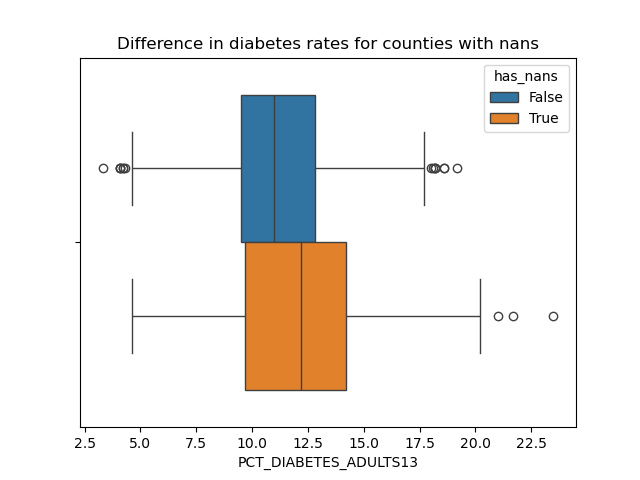
\includegraphics[width=0.75\linewidth]{figures/diabetes rates vs nans boxplot.png}
            \caption{Diabetes rates are higher in counties with incomplete data}
        \end{figure}

    \pagebreak
    \item \textbf{\textit{Detrending model}}
            \label{fig:detrend}
        \begin{figure}[h!]
            \centering
            \includegraphics[width=1\linewidth]{figures/detrend.png}
            \caption{Health Score vs all income and age structure features. Predictions from this model were used to detrend Health Score for future models.}
        \end{figure}

    \pagebreak
    \item \textbf{\textit{LassoCV alpha}}
            \label{fig:lassocv}
    
        Graphic code from: \url{https://scikit-learn.org/stable/auto_examples/linear_model/plot_lasso_model_selection.html#sphx-glr-auto-examples-linear-model-plot-lasso-model-selection-py}
        \begin{figure}[h!]
            \centering
            \includegraphics[width=0.75\linewidth]{figures/lassocv coordinate descent.png}
            \caption{LASSO 10-fold cross validation alpha selection}
        \end{figure}

    \pagebreak
    \item \textbf{\textit{Statsmodels OLS results}}
            \label{fig:statsmodelsOLS}
        \begin{figure}[h!]
            \centering
            \includegraphics[width=1\linewidth]{figures/statsmodels ols results.png}
            \caption{Statsmodels OLS results. Detrended health score vs normalized features.}
        \end{figure}

    \pagebreak
    \item \textbf{\textit{RandomForestRegressor Gini importance}}
             \label{fig:enter-label}
       \begin{figure}[h!]
            \centering
            \includegraphics[width=0.75\linewidth]{figures/gini_importance.png}
            \caption{Random Forest Gini importance. Detrended health score vs normalized features.}
        \end{figure}

    \pagebreak
    \item \textbf{\textit{Race/ethnicity k-means scores}}
            \label{fig:kmeans_scores}
        \begin{figure}[h!]
            \centering
            \includegraphics[width=0.75\linewidth]{figures/cluster_scores.png}
            \caption{K-means clustering scores by number of clusters}
        \end{figure}

    \pagebreak
    \item \textbf{\textit{Race/ethnicity cluster distributions}}
             \label{fig:kmeans_pairplot}
       \begin{figure}[h!]
            \centering
            \includegraphics[width=0.75\linewidth]{figures/cluster_pairplot.png}
            \caption{K-means clustering with 3 clusters seems to partition the data effectively}
        \end{figure}

    \pagebreak
    \item \textbf{\textit{Urban vs rural counties}}
            \label{fig:urban_rural}
        \begin{figure}[h!]
            \centering
            \includegraphics[width=0.75\linewidth]{figures/urban vs rural.png}
            \caption{Urban counties are healthier and more populated (by median)}
        \end{figure}

    \pagebreak
    \item \textbf{\textit{Income and race/ethnicity}}
            \label{fig:income_race}
        \begin{figure}[h!]
            \centering
            \includegraphics[width=1\linewidth]{figures/race vs income.png}
            \caption{Median household income by race/ethnicity}
        \end{figure}

    \pagebreak
    \item \textbf{\textit{Health and race/ethnicity}}
            \label{fig:health_race}
        \begin{figure}[h!]
            \centering
            \includegraphics[width=1\linewidth]{figures/race vs health.png}
            \caption{Health Score by race/ethnicity}
        \end{figure}

    \pagebreak
    \item \textbf{\textit{Age structure and chronic disease}}
            \label{fig:age_chronic}
        \begin{figure}[h!]
            \centering
            \includegraphics[width=0.75\linewidth]{figures/chronic disease vs age structure.png}
            \caption{Counties with older populations have higher diabetes rates and counties with younger populations may have higher heart disease mortality}
        \end{figure}

    \pagebreak
    \item \textbf{\textit{Healthy store access by racial/ethnic cluster}}
            \label{fig:cluster_store_access}
        \begin{figure}[h!]
            \centering
            \includegraphics[width=1\linewidth]{figures/store_access_clusters.png}
            \caption{There are no clear trends regarding healthy store access and racial/ethnic clusters.}
        \end{figure}
\end{enumerate}

\end{itemize}


\end{document}

